\chapter{Logik und Unterlagen}
Im Laufendes Semester werden wir viele mathematische Beweise einführen. Heute werden wir uns mit der Mathematische Logik beschäftiges.\\

In Mathematik stutzen wir uns auf gewisse Grundannahmen ``Axiome'', die wir als gegeben ansehen. Eine dieser Annahmen ist der 
\subsection*{Satz von ausgeschlossenen Dritten}
Eine zulässige mathematische Aussage ist entweder wahr oder falsch, jedoch nie beiden zugleich.
\subsubsection*{Beispiel}
\begin{enumerate}
	\item $5<7$ Wahr
	\item $4<2$ Falsch
\end{enumerate}
In der Wirklichen Welt ist es anders , z.B. ``Mathematik ist schön'', wahr oder falsch?\\

Mit Aussagen kann man ``rechnen''. Wir führen nun ein Paar \todo{??gehäufige?? Page 1} Notationen der Logik ein:\\
Seien $A,B$ Aussagen
\begin{itemize}
\item $A$ und $B$ wird mit $A\land B$ bezeichnet
\item $A$ oder $B$ wird mit $A\lor B$ bezeichnet
\end{itemize}
\subsubsection*{Folgerung (eine wahre implikation)}
\begin{itemize}
\item Aus $A$ folgt $B$ wird mit $\Rightarrow$ bezeichnet
\item Wenn $A$, dann $B$ wird mit \todo{Cannot read, page 2 middle}
\item Die negation der Aussage $A$ wird mit $\lnot A$ bezeichnet
\item $A$ ist equivalent zu $B$ wird mit $A\Leftrightarrow B$ bezeichnet
\item $\left(A\Rightarrow B\right)\land \left( B\Rightarrow A\right)$ $A$ wahr genau dann, wenn $B$ wahr ist.
\end{itemize}

\subsubsection*{Bemerkung}
Die Folgerung ist transitive. Wir wissen $A\Rightarrow B$ und $B\Rightarrow C$, dann wissen wir dass $A\Rightarrow C$.

\subsection*{Prinzip der Mathematischen Beweises}
Wir können ber eine Kette von Folgerungen \[A\Rightarrow B \Rightarrow C \dots \Rightarrow S\]
einen mathematischen ``Satz'' $S$ aus einen annahme $A$ herleiten. (Ein Beweis ist eine Folge von Implikationen von Aussagen). 
\subsubsection*{Kontroposition (Umkehrschluss)}
$A\Rightarrow B$ ist gleichbedeutend mit $\lnot B\Rightarrow\lnot A$.\\
Falls $A\Rightarrow B$, so kann $A$ nicht wahr sein wenn $B$ falsch ist (weil $A$ wahr wäre, würde $B$ auch wahr sein).

\section{Prinzip des Indirekten Beweises}
Zum Beweis der Aussage $A\Rightarrow B$ genügt es die Aussage $\lnot B\Rightarrow\lnot A$ zu zeigen, oder: die Annahme $A\land\lnot B$ zum Wiederspruch zu führen.

\subsection*{Indirekten Beweis}
Man fügt $\lnot B$ als Annahme hinzu und kommt nach einer Kette von erlaubten schlüssen zu einer falschen Aussage.\\

\noindent Hieraus schliesst man, dass das zusatzannahme $\lnot B$ nicht wahr ist. 

\subsubsection*{Beispiel 1.1}
\begin{itemize}
\item $A=\text{''jede natürliche Zahl } n \text{ hat einen Nachfolger } n+1\text{''}$
\item $B=\text{''es gibt keine grösste Naturliche Zahl''}$
\end{itemize}

\noindent Wir beweisen dass aus $A$ folgt $B$. Nehmen wir an, dass $A$ wahr und $B$ falsch ist. \\

\noindent $\lnot B=$ es gibt eine grösste Natürliche zahl$N_0''$ d.h $N_0>l$ für jedes $l \in \mathbb{N}$.\\

Mittels der Aussage $A$ wissen wir dass $N_0$ einen Nachfolger $N_0 +1$ hat. Dann $N_0+1>N_0$. Dass ist ober ein Wiederspruch.

\begin{definition}{1.1}
Eine Menge ist eine Zusammenfassung verschiedener Objekte zu einem Ganzen.\\
Die Objekte werden Elemente der Menge genannt. 
\end{definition}

Sei $A$ eine Menge, dann ``$a$ ist element von $A$'' wird mit ``$a\in A$'' bezeichnet.\\
Seien $A,B$ Mengen, dann ``jedes Element von $A$ ist ein Element von $B$'' wird mit ``$A\subset B$ bezeichnet, und man sagt ``$A$ ist in $B$ enthalten'' (oder $A$ ist teilmenge von $B$). \\

Falls zugleich $A\subset B$ und $B\subset A$ gilt, bezeichnet man $A$ und $B$ als gleich und schreibt $A=B$. 

\subsubsection*{Beispiele 1.2}
\begin{enumerate}
	\item Die Menge $\mathbb{N}=\{0,1,2,\dots\}$ der Natürlichen zahlen.
	\item Die leere Menge mit ``$\varnothing$'' bezeichnet. Sie ist in jeder Menge enthalten.
	\item Die Menge $\mathbb{Z}=\{\dots,-2,-1,0,1,2,\dots\}$ aller ganze Zahlen.
	\item Meistens werden Mengen nicht durch die Liste ihre Elemente gegeben, sondern durch bestimmte Eigenschaften ihrer Elemente definiert \[\mathbb{P}=\{2,3,4,5,7,11,13,\dots\}\] die Menge aller Primzahlen $\mathbb{P}:\{p\in\mathbb{N}\mid\text{ $p$ primzahl}\}$
\end{enumerate}
\section{Zwei Prinzipen}
Wir werden 2 Methoden des Beweises häufig benutzen.

 \subsection*{1. Prinzip des Indirekten Beweises}
Zum Beweis der Aussage $A\Rightarrow B$ genügt es die Aussage $\lnot B\Rightarrow\lnot A$ zu zeigen, oder, die Annahme $A\land\lnot B$ zum Wiederspruch zu führen.
\subsection*{2. Prinzip der Vollständigen Induktion}
Sei für jedes $n\in\mathbb{N}$ eine Behauptung $A(n)$ gegeben. Soll die Behauptung für alle natürlichen Zahlen $n\in\mathbb{N}$ bewiessen werden so genügen dazu zwei Beweisschritte:
\begin{enumerate}[i)]
\item Der Beweis von $A(0)$
\item Für jedes $n\in\mathbb{N}$, der Beweis von $A(n+1)$ unter der Voraussetzung, dass $A(n)$ gilt. 
\end{enumerate}
Oft Behauptungen nicht von $n=0$ antreten. \\
Soll die Gültigkeit von $A(n)$ für alle $n\geq m$ bewiesen werden so genügen wieder zwei Schritte:
\begin{enumerate}[i)]
	\item Beweis von $A(m)$
	\item Für jedes $n\geq m$ impliziert $A(n)$ die Behauptung $A(n+1)$
\end{enumerate}
Das Prinzip der Vollständige Induktion ist genau wie ein Dominoeffekt.\\

Sie stellen alle Dominosteinen eine nach der andere. Falls der erste Dominostein füllt ($A(1)$ wahr) und falls wir die Dominosteinen genug nebeneinander gestellt haben, so dass ein fallender Dominostein den nächsten trifft ($A(k)\Rightarrow A(k+1)$) dann wissen wir, dass alle Dominosteinen fallen. 

\subsubsection*{Beispiel 1.3 (Induktion)}
\begin{enumerate}
\item Für alle $n\geq 1$ gilt: \[1+3+5+\dots (2n-1)=n^2\text{\indent\indent}A(n)\] Beweis mittels Vollständige Induktion
\begin{enumerate}[i)]
\item $A(i)$ lautet $1=1^2$ und gilt.
\item Sei $n\geq 1$. Annahme: so gilt $A(n)$. Die Linke Seite der Identität $A(n+1)$ ist \[1+3+\dots (2n-1)+(2n+1)=n^{2}+(2n+1)=(n+1)^2\] womit $A(n+1)$ bewiesen ist.
\end{enumerate}
\item Als zweite Beispiel für Vollständige Induktion beweisen wir den Fundamental Satz von Euklid:
\subsubsection*{Satz 1.4}
Jede Natürliche Zahl $n\geq 2$ ist ein Produkt von Primzahlen, dass bis auf die Reihenfolge der Faktoren eindeutig ist. Wir werden uns hier nicht mit der eindeutigkeit befessen.
\subsubsection*{Beweis}
Sei $A(n)$ die Aussage: Jede Natürliche Zahl $m$ mit $2\leq m\leq n$ ist ein Produkt von Primzahlen
\begin{enumerate}[i)]
\item $A(2)$ gilt denn $2$ ist Primzahl
\item Sei $n\geq 2$. Wir nehmen an, dass $A(n)$ gilt. Für $n+1$ gibt es zwei Möglichkeiten
\begin{enumerate}[a)]
\item $n+1$ ist eine Primzahl und somit gilt $A(n+1)$ 
\item $n+1$ ist keine Primzahl d.h. es gibt $2\leq a\leq n$ die $n+1$ teilt. Dann ist $b:=\frac{n+1}{a}$ auch ganz und zudem erfüllt $2\leq b\leq n$ . Aus $A(n)$ folgt dass sowohl $a$ wie $b$ ein Produkt von Primzahlen sind somit $n+1=ab$ ein product von Primzahlen ist. 
\end{enumerate}
\end{enumerate}
\end{enumerate}
\subsubsection*{Satz 1.5}
Die Menge $\mathbb{P}$ der Primzahlen ist unendlich.
\subsubsection*{Beweis}
Nehmen wir an das gegenteil ``$\mathbb{P}$ ist endlich'', d.h. $\mathbb{P}=\{p_1,p_2,\dots,p_m\}$ n aufsteigender Folge; also $p_1=2,p_2=3,p_3=5,p_4=7,\dots$. Wir betrachten die Zahl $k=p_1\dots p_{m+1}$. Auf Satz 1.4 folgt dass so eine Primzahl $p_i$ (aus der liste $p_1\dots p_{m}$) gilt mit $p_i$ teilt $k$. Da $p_i$ offensichtlich $p_1\dots p_{m}$ teilt, folgt dass $p_i$ $k-p_1\dots p_{m}=1$ teilt. Das ist ein Widerspruch. 

\subsection*{Teilbarkeit}
\subsubsection{Formale Definition}
Eine Ganze Zahl $a$ teilt eine ganze Zahl $b$ genau dann, wenn es eine ganze Zahl $n$ gibt, für die $an=b$ ist. \\
\todo{Please fill out the table}
\begin{center}
\begin{tabular}{l|l}
Man sagt dann & Man schreibt \\\hline 
$a$ teilt $b$ & $a\mid b$\\
$a$ ist teiler von $b$ & ~\\
$b$ ist teilbar durch $a$ & ~\\
$b$ ist Vielfaches durch $a$ & ~\\
\end{tabular}
\end{center}

\subsubsection*{Eigenschaften der Teilbarkeit}
\begin{itemize}
\item Gilt $a\mid b$ und $b\mid c$, so folgt $a\mid c$
\item Für $k\in\mathbb{Z}\backslash\{0\}$ gilt: $a\mid b\Longleftrightarrow ka\mid kc$ 
\item $a\mid b$ und $c\mid d\Rightarrow ac\mid bd$
\item $a\mid b$ und $a\mid c\Rightarrow a\mid kb+lc,\text{    für alle }l,k\in\mathbb{Z}$
\end{itemize}

\begin{enumerate}
\item $k=\left( p_1 p_2\dots p_i \dots p_m \right)+1$\\
Es gibt eine Primzahl $p_i$ dass $k$ teilt. $p_i\mid k$ mittels Satz 1.4.
\item Sei $b=p_1 p_2\dots p_i \dots p_m=$ produkt aller Primzahlen. Sei $a=p_i$, $n=p_1 p_2 p_{i-1} p_{i+1} \dots p_m$. Dann $b=an$. Dass heisst $a$ ist Teiler von $b$, d.h. $p_i\mid\left(p_1\dots p_m\right)$
\item $p_i\mid k$ und $p_i\mid \left(p_1\dots p_m\right) \Rightarrow p_i \mid k-\left(p_1\dots p_m\right)=1$.\\
So erhalten wir einen Wiederspruch
\end{enumerate}

\subsubsection*{Bemerkung}
Letztes mal haben wir gesagt jedes element von $A$ ist auch Element von $B$ ($\forall x,x\in A\Rightarrow x\in B$) wird mit $A\subset B$ ($A$ ist in $B$ enthalten, $A$ ist Teilmenge von $B$) bezeichnet. Falls $A\subset B$ und eine Element $b\in B$ gibt mit $b\not\in A$ sagen wir $A$ ist eine ``eigentliche Teilmenge'' von $B$. Manchmal schreiben wir $A\mathop  \subset \limits_{\not  = } B$ in diesem Fall. \\

Es gibt viele Bücher, mit der Folgenden Notation: jedes element von $A$ ist ein element von $B$ wird mit $A\subseteq B$ bezeichnet. Und wenn $A\subseteq B$ und $A\not =B$ dann benutzen sie $A\subset B$ statt $A\mathop  \subset \limits_{\not  = } B$. $A=B$ falls $x\in A\Leftrightarrow x\in B$. 

\subsubsection*{Satz}
$A=B \Leftrightarrow A\subset B$ und $B\subset A$ 
\subsubsection*{Beweis}
Annahme: $A=B$. Falls $x\in A$, dann mittels $A=B$, $x\in B$ gilt, damit gilt $A\subset B$ und falls $x\in B$, dann $x\in A$ gilt (mittels $A=B$) damit gilt $B\subset A$.\\

Wir haben bewiesen dass $A=B \Rightarrow A\subset B \text{ und } B\subset A$. Zunächst nehmen wir an dass $A\subset B$ und $B\subset A$. Wir möchten zeigen dass $A=B$. \\

Sei $x\in A$, mittels $A\subset B$, haben wir $x\in B$ somit $x\in A \Rightarrow x\in B$. (\textasteriskcentered)\\

Sei $x\in B$, mittels $B\subset A$, haben wir $x\in A$ somit $x\in B \Rightarrow x\in A$. (\textasteriskcentered\textasteriskcentered)\\

(\textasteriskcentered) und (\textasteriskcentered\textasteriskcentered) $\Rightarrow A=B$ per Definition. 

\section{Mengeoperationen}
Zunächst erinnern wir kurz an die Definitionen der Elementaren Operationen auf Mengen. \\

\noindent Seien $A$ und $B$ Mengen. Wir können dann daraus folgende Mengen bilden:

\begin{itemize}
\item Die Vereinigung: $A\cup B=\{x\mid x\in A \text{ oder } x\in B\}$
\item Der Durchschnitt: $A\cap B=\{x\mid x\in A \text{ und } x\in B\}$
\item Die Differenz: $A\backslash B=\{x\mid x\in A \text{ und } x\not\in B\}$
\item Symmetrische Differenz: $A\bigtriangleup B=\left(A\backslash B\right) \cap \left(B\backslash A\right)=\left(A\cup B\right)\backslash\left(A\cap B\right)$
\end{itemize}

Wir haben dann folgende Eignschaften
\subsubsection*{Satz 1.6}
Seien $A,B,C$ Mengen. 
\begin{enumerate}
\item $A\cap B=B\cap A$; $A\cup B=B\cup A$\\
$A\cap \emptyset=\emptyset$; $A\cup \emptyset=A$\vspace{-4mm}
\subsubsection*{Bemerkung}
\begin{itemize}
    \item $\cup$ verhaltet sich wie $+$
    \item $\cap$ verhaltet sich wie Multiplikation
    \item $\emptyset$ verhaltet sich wie Null element
\end{itemize}
    \item $\left( A\cup B\right)\cup C=A\cup\left( B\cup C\right)$\\
    $\left( A\cap B\right)\cap C=A\cap\left( B\cap C\right)$
    \item $\left( A\cup B\right) \cap C=\left( A\cap C\right) \cup \left( B\cap C\right)$
\end{enumerate}



\subsubsection*{Beweis}
Übung \todo{Ask for correct beweis!!}

\begin{definition}{1.7}
Das Kartesische Produkt $A\times B$ der Mengen $A,B$ ist die Menge der geordneten Paare $(a,b)$ wobei $a\in A, b\in B$
\end{definition}

\subsubsection*{Beispiel}
$\mathbb{Z}\times\mathbb{Z}=\{(a,b):a\in\mathbb{Z},b\in\mathbb{Z}\}$. Falls $\mathbb{Z}$ als ``eindimensionalen'' Gebilde dargestellt wird 

\begin{center}
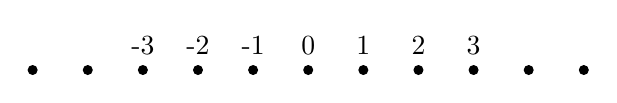
\begin{tikzpicture}[scale=0.7]


\draw	(0,0) node[anchor=south] {-3}
		(1,0) node[anchor=south] {-2}
		(2,0) node[anchor=south] {-1}
		(3,0) node[anchor=south] {0}
		(4,0) node[anchor=south] {1}
		(5,0) node[anchor=south] {2}
		(6,0) node[anchor=south] {3}
		
		;
\filldraw (2,-0.1) circle (0.08)
(1,-0.1) circle (0.08)
(0,-0.1) circle (0.08)
(-1,-0.1) circle (0.08)
(-2,-0.1) circle (0.08)
(2,-0.1) circle (0.08)
(3,-0.1) circle (0.08)
(4,-0.1) circle (0.08)
(5,-0.1) circle (0.08)
(6,-0.1) circle (0.08)
(7,-0.1) circle (0.08)
(8,-0.1) circle (0.08)
;
		
		
\end{tikzpicture}
\end{center}


so wird $\mathbb{Z}\times\mathbb{Z}$ als ``zweidimensionalen'' Gebilde dargestellt 

\begin{center}
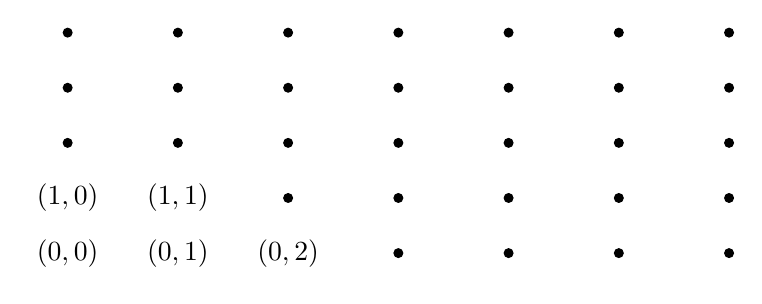
\begin{tikzpicture}[scale=0.7]


\draw	(0,0) node[] {$(0,0)$}
		(2,0) node[] {$(0,1)$}
		(4,0) node[] {$(0,2)$}
		(0,1) node[] {$(1,0)$}
		(2,1) node[] {$(1,1)$}
		;
\filldraw 
(0,2) circle (0.08)
(0,3) circle (0.08)
(0,4) circle (0.08)
(2,2) circle (0.08)
(2,3) circle (0.08)
(4,3) circle (0.08)
(6,3) circle (0.08)
(8,3) circle (0.08)
(10,3) circle (0.08)
(12,3) circle (0.08)
(4,2) circle (0.08)
(6,2) circle (0.08)
(8,2) circle (0.08)
(10,2) circle (0.08)
(12,2) circle (0.08)

(4,1) circle (0.08)
(6,1) circle (0.08)
(8,1) circle (0.08)
(10,1) circle (0.08)
(12,1) circle (0.08)
(10,0) circle (0.08)
(12,0) circle (0.08)

(2,4) circle (0.08)
(4,4) circle (0.08)
(6,4) circle (0.08)
(8,4) circle (0.08)
(10,4) circle (0.08)
(12,4) circle (0.08)
(6,0) circle (0.08)
(8,0) circle (0.08)
;
\end{tikzpicture}
\end{center}



Um die Operationen auf mehrere Mengen zu Verallgemeinern sind die folgenden Quantoren nützlich ($\ast$)
\begin{enumerate}
\item $\forall$ ``Für alle'' (Allquantor)
\item $\exists$ ``Es gibt'' (Existenzquantor)
\item $\exists !$ ``Es gibt genau ein''
\end{enumerate}
Sei nun $I$ eine beliebige Menge ($I$=Indexmenge) und sei für alle $i\in I$ eine Menge $A_i$ gegeben. Dann:
\begin{itemize}
\item $\mathop { \cup {A_i}}\limits_{i \in I} = \{x\mid \exists i\in I,x\in A_i\}$. Vereinigung besteht aus den Elementen $x$, für welche eine $i\in I$ gibt so dass $x$ zu $A_i$ gehört.
\item  $\mathop { \cap {A_i}}\limits_{i \in I} = \{x\mid \forall i\in I,x\in A_i\}$. Durchschnitt. 
\end{itemize}
Wir \todo{?löhnen? page 15} noch das Kartesische Produkt endlich vieler Mengen $A_1 \dots A_n$ definiere \[{A_1} \times {A_n} = \prod\limits_{i = 1}^n {{A_i} = \{ ({x_1} \ldots {x_n})\mid {x_i} \in {A_i}} \} \]

\subsubsection*{Satz 1.8}
Seien $A_1 \dots A_k \subset x,k\in \mathbb{N}$. Es gilt
\begin{enumerate}
\item \[{\left( {\bigcap\limits_{i = 1}^k {{A_i}} } \right)^c} = \bigcup\limits_{i = 1}^k {{A_i}^c} \]
\item \[{\left( {\bigcup\limits_{i = 1}^k {{A_i}} } \right)^c} = \bigcap\limits_{i = 1}^k {{A_i}^c} \]
\end{enumerate}
\begin{enumerate}[($\ast$)]
\item Wir haben gesehen dass wir manchmal eine Aussage verneinen müssen. Deshalb müssen wir lernen wie man Aussage mit Quantoren verneinen kann.
\[\neg\left(\forall n:A(n)\right)\Leftrightarrow\left(\exists n:\neg A(n)\right)\]
\[\neg\left(\exists n:A(n)\right)\Leftrightarrow\left(\forall n:\neg A(n)\right)\]
\[\neg\left(\forall x\in \mathbb{R}:x^2\geq 0\right)\Leftrightarrow\exists x\in\mathbb{R}:x^2<0\]
\end{enumerate}
\section{Abbildungen}
Seien $X,Y$ Mengen. 

\begin{definition}{1.9}
Eine Funktion oder Abbildung $f:X\rightarrow Y$ der Menge $X$ in die Menge $Y$ ist eine Vorschrift (ein Gesetz) die (das) jedem Element $x\in A$ genau ein Element $y=f(x)\in Y$ zuordnet. \\

Es gibt verschiedene wichtige Objekte die in Zusammenhang mit einem Abbildung auftreten 
\[X= \text{ Definitionsbereich von } f\]
\[Y= \text{ Die Ziel Menge}\]
\[f(x)=\{f(x)\mid x\in X\}\text{ ist das Bild von }f\text{ oder die Bildmenge}\]
\end{definition}

\subsubsection*{Beispiel 1.10}
\begin{enumerate}
\item (Identität) Für jede Menge $\Romanbar{X}$, ist $id_X : \Romanbar{X} \rightarrow\Romanbar{X}$ definiert durch $id_{\Romanbar{X}}(x)=x, \forall x\in X$ 

\begin{center}
\begin{tikzpicture}[scale=0.5]
\draw (-2.5,0) ellipse (1.5 and 3);
\draw (2.5,0) ellipse (1.5 and 3);


\draw[-triangle 60]  (-2.5,2) parabola bend (-0.5,2) (2.8,1.3);


\draw[-triangle 60](-2.8,0) parabola bend (1,1) (3.2,0.5);
\draw[-triangle 60](-2,-1) parabola bend (0,-0.8) (2,-1);

\draw	(-1,3) node[anchor=east] {$X$}
		(4,3) node[anchor=east] {$X$};



\filldraw 
(-2.5,2) circle (0.08)
(-2.8,0) circle (0.08)
(-2,-1) circle (0.08)

(2.8,1.3) circle (0.08)
(3.2,0.5) circle (0.08)
(2,-1) circle (0.08)
;
\end{tikzpicture}
\end{center}



\item (Konstante) Sei $X$ Menge und $c\in \Romanbar{X}$. Die konstante Abbildung mit wert $c$ ist $f(x)=c, \forall x \in \Romanbar{X}$  

\begin{center}
\begin{tikzpicture}[scale=0.5]
\draw (-2.5,0) ellipse (1.5 and 3);
\draw (2.5,0) ellipse (1.5 and 3);


\draw[-triangle 60]  (-2.5,2) parabola bend (-0.5,2) (3.2,0.5);


\draw[-triangle 60](-2.8,0) parabola bend (1,1) (3.2,0.5);
\draw[-triangle 60](-2,-1) parabola bend (3.2,0.5) (3.2,0.5);

\draw	(-1,3.1) node[anchor=east] {$\Romanbar{X}$}
		(4,3.1) node[anchor=east] {$\Romanbar{X}$}
		(3.9,0.1) node[anchor=east] {$C$}
		;

\filldraw 
(-2.5,2) circle (0.08)
(-2.8,0) circle (0.08)
(-2,-1) circle (0.08)


(3.2,0.5) circle (0.08)
;
\end{tikzpicture}
\end{center}


\item Seien $X,Y$ Mengen. Dann sind \\
\begin{tabular}{r  l c r l c }
$pr_x:$ & $X\times Y\rightarrow X $& ~ & $pr_y$: & $X\times Y\rightarrow Y$ \\
~& $(x,y)\rightarrow x$ & ~& ~& $(x,y)\rightarrow y$ \\
\end{tabular}\\
die Projektionen auf dem ersten respektiv zweiten Faktoren. 
\item $f:\mathbb{R}\rightarrow\lbrack -1,1\rbrack$\\ $x\rightarrow \sin x$
\item $f:\mathbb{R}\rightarrow\mathbb{R}$\\
$x\rightarrow x^2+x$
\end{enumerate}
\begin{definition}{1.11}
Sei $f:X\rightarrow Y$ eine Abbildung
\begin{enumerate}
\item $f$ heisst injektiv falls auf $f(x_1)=f(x_2)$ stets $x_1=x_2$ folgt, falls jeder $y<\in Y$ höchstens ein Urbild hat.
\item $f$ heisst surjektiv falls für jedes $y\in Y$ ein $x\in X$ gibt mit $f(x)=y$ \[\forall y\in Y, \exists x\in X:f(x)=y\]wenn jedes Element $y\in Y$ mindestens ein Urbild hat. 
\item $f$ heisst bijektiv falls $f$ injektiv und surjektiv ist, d.h. falls jedes $y\in Y$ genau ein Urbild hat. 
\end{enumerate}
\end{definition}

\todo{Pages from 17.1 to 17.4 seem repetition, ask to be sure (document week2)}

\subsubsection*{Beispiel 1.12}
\todo{WRONG POSITION!!}
\begin{figure}[ht]

\begin{minipage}[b]{0.45\linewidth}
\centering
\begin{enumerate}
\item $id_{X}:X\rightarrow X$ bijektive.
\item Eine konstante Abbildung $f:X\rightarrow X, x\rightarrow c$ ist 
\begin{itemize}
\item bijektive $\Leftrightarrow \Romanbar{X}=\{ c\}$
\item surjektive $\Leftrightarrow \Romanbar{X}=\{ c\}$
\end{itemize}
\item Die Projektionen 
\begin{itemize}
\item $pr_x : X\times Y\rightarrow X$ 
\item $pr_y : X\times Y\rightarrow Y$ 
\end{itemize}
sind stets surjektive.
\item $f:\mathbb{R}\rightarrow\lbrack -1,1\rbrack$ \\
$x\rightarrow \sin x$\\
Surjektiv, nicht injektiv
\end{enumerate}
\end{minipage}
\hspace{0.5cm}
\begin{minipage}[b]{0.45\linewidth}
\centering
\begin{enumerate}
\item $f:\mathbb{R}\rightarrow\mathbb{R}$\\
$x\rightarrow x^2$\\
Nicht surjektiv\\
Nicht injektiv

\item $f:\mathbb{N}\rightarrow\mathbb{N}$\\
$n\rightarrow 2n$\\
ist Injektive. $f(\mathbb{N})$ ist die Menge aller geraden Zahlen
\item Eine Menge $A$ hat $n$ Elemente falls es eine bijektive $f:\{1,\dots,n\}\rightarrow A$ gibt. Die Zahl $n$ wird dann die Kardinalität von $A$ genannt und mit  bezeichnet, gelegentlich auch mit $\#A$ bezeichnet


\end{enumerate}
\end{minipage}
\end{figure}

\todo{unreadeable, page 18}

\begin{definition}{Kardinalität}
Wir sagen zwei Mengen $X$ und $Y$ sind gleichmächtig falls eine bijektive Abbildung $f:X\rightarrow Y$ gibt.
\end{definition}

Mit dem ersten Contorschen Diagonalverfahren kann man die Rationalen zahlen abzählen, d.h.$ \mathbb{Q}$ und $\mathbb{N}$ sind gleichmächtig

\begin{center}
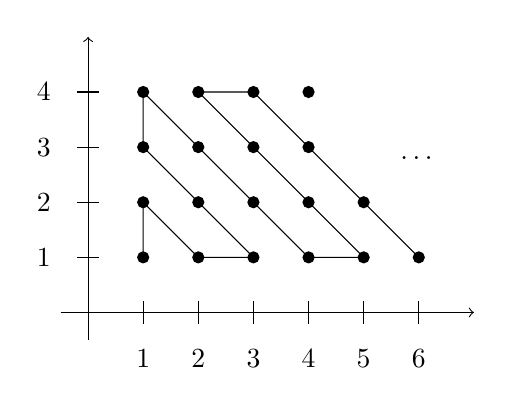
\begin{tikzpicture}[scale=0.7]

% horizontal axis
\draw[->] (-0.5,0) -- (7,0) node[anchor=north] {};
% labels
\draw	(-0.5,1) node[anchor=east] {1}
		(-0.5,2) node[anchor=east] {2}
		(-0.5,3) node[anchor=east] {3}
		(-0.5,4) node[anchor=east] {4}
		
		(1,-0.5) node[anchor=north] {1}
		(2,-0.5) node[anchor=north] {2}
		(3,-0.5) node[anchor=north] {3}
		(4,-0.5) node[anchor=north] {4}
		(5,-0.5) node[anchor=north] {5}
		(6,-0.5) node[anchor=north] {6}
		
		(6,3) node[anchor=north] {\dots}
		
		;
%lines for labes
\draw (-0.2,1) -- (0.2,1)
(-0.2,2) -- (0.2,2)
(-0.2,3) -- (0.2,3)
(-0.2,4) -- (0.2,4)

(1,-0.2) -- (1,0.2)
(2,-0.2) -- (2,0.2)
(3,-0.2) -- (3,0.2)
(4,-0.2) -- (4,0.2)
(5,-0.2) -- (5,0.2)
(6,-0.2) -- (6,0.2);

%draw dots
\filldraw[color=black] (1,1) circle (0.1)
(2,1) circle (0.1)
(3,1) circle (0.1)
(4,1) circle (0.1)
(5,1) circle (0.1)
(6,1) circle (0.1)
(1,2) circle (0.1)
(2,2) circle (0.1)
(3,2) circle (0.1)
(4,2) circle (0.1)
(5,2) circle (0.1)
(1,3) circle (0.1)
(2,3) circle (0.1)
(3,3) circle (0.1)
(4,3) circle (0.1)
(1,4) circle (0.1)
(2,4) circle (0.1)
(3,4) circle (0.1)
(4,4) circle (0.1)
;

% vertical axis
\draw[->] (0,-0.5) -- (0,5) node[anchor=east] {};

%connection through points
\draw (1,1)--(1,2)--(2,1)--(3,1)--(2,2)--(1,3)--(1,4)--(4,1)--(5,1)--(2,4)--(3,4)--(6,1);

% Psis

\end{tikzpicture}
\end{center}
\section{Dedekind Schubladen Prinzip}\todo{Is this supposed to be a new chapter?? page 19}
Sei $f:A\rightarrow B$ eine beliebige Abbildung zwischen endliche Mengen. Falls $\left| B\right| < \left| A \right|$ dann ist $f$ nicht injektiv, d.h. es gibt $b\in B$ und $a_1,a_2\in A$ mit
\begin{enumerate}[i)]
\item $a_1\not=a_2$
\item $f(a_1)=f(a_2)=b$
\end{enumerate}

\begin{center}
\begin{tikzpicture}[scale=0.5]
\draw (-2.5,0) ellipse (1.5 and 3);
\draw (2.5,0) ellipse (1.5 and 3);


\draw[-triangle 60]  (-2.5,2) parabola bend (-0.5,2) (2.8,1.3);


\draw[-triangle 60](-2.8,0) parabola bend (1,1) (3.2,0.5);
\draw[-triangle 60](-2,-1) parabola bend (0,-0.8) (2,-1);
\draw[-triangle 60](-3,1.5) parabola bend (0,1.8) (3.2,0.5);
\draw[-triangle 60](-2.3,-2) parabola bend (0,-3) (2.1,-2.9);



\draw	(-1,3) node[anchor=east] {$A$}
		(0.5,2.5) node[anchor=east] {$f$}
		(4,3) node[anchor=east] {$B$};



\filldraw 
(-2.5,2) circle (0.08)
(-2.8,0) circle (0.08)
(-2,-1) circle (0.08)
(-3,1.5) circle (0.08)
(-2.3,-2) circle (0.08)


(2.8,1.3) circle (0.08)
(3.2,0.5) circle (0.08)
(2,-1) circle (0.08)
;
\end{tikzpicture}
\end{center}
\centerline{$3=\left| B\right| < 5 = \left| A \right|$}

Mit Abbildungen kann man ``operieren''. Die wichstige Operation ist die Verkettung (oder komposition) zweier Abbildungen. 

\begin{definition}
\noindent Abbildungen $f:X\rightarrow $, $g:Y\rightarrow Z$ kann man miteinander ausführen. Dies ergibt eine neue Abbildung \[X\mathop  \to \limits^f Y\mathop  \to \limits^g Z\] \[F:=g\circ f:X\rightarrow Z, x\rightarrow g\left( f(x)\right)   \]
\end{definition}
Zwei Funktionen $f$ und $g$ können verkettet werden wenn der Wertebereich der ersten Funktion mit dem Definitionsbereich der zweiten Funktion übereinstimmt. 

\[\text{Man Sagt}\left\{ {\begin{array}{*{20}{c}}
{g\text{ nach }f\text{ oder }}\\
{g\text{ komponiert mit }f}\\
{g\circ f}
\end{array}} \right.\]

\underline{Zu Beachten:}
In dieser Notation steht die zuerst angewandte Abbildung rechts; das heisst bei $g\circ f$ wird zuerst die Funktion $f$ angewandt und dann die Funktion $g$. 
\begin{itemize}
\item Die Identische Abbildung verhölt sich bei der Komposition \todo{?neu?, page 19.2 top}, für eine Funktion \[f:X\rightarrow Y \text{ gilt also}\]
\[f\circ id_X=f=id_Y \circ Y\] wobei \[id_X:\Romanbar{X}\rightarrow\Romanbar{X}\]\[x\rightarrow x\] \[id_Y :Y\rightarrow Y\]\[y\rightarrow y\]

\item Die Komposition von Funktionen ist associativ, d.h. für Funktionen $f,g,h$ gilt \[\left( h\circ g\right)\circ f=h\circ \left( g\circ f\right)\]
\item Aber die Komposition von Funktionen ist im Allgemeinen nicht kommutativ! \[f\circ g\not= g\circ f\]
Zum Beispiel:
\[f:\mathbb{R}\rightarrow\mathbb{R}\]\[x\rightarrow x^2\]\[g:\mathbb{R}\rightarrow\mathbb{R}\]\[x\rightarrow x+1\]
\[f\circ g=f\left( g(x)\right)=f(x+1)=(x+1)^2=x^2+2x+1\]\[g\circ f=g\left( f(x)\right)=g(x^2)=x^2+1\]
\end{itemize}

\section{Die Inverse Abbildung (Umkehrfunktion)}
Sei $f:X\rightarrow Y$ eine bijektiven Funktion. \\

Die Inverse Funktion $g:Y\rightarrow X$, einer bijektiven Funktion $f:X\rightarrow Y$ ist die Funktion, die jedem Element $y$ der Zielmenge seien eindeutig bestimmtes Urbildelement zuweist. (bei bijektiven Funktionen hat die Urbildmenge jedes Element $y$ genau ein Element). \\

 $g(y):=x$, eindeutig definierte $ x\in\Romanbar{X}$, mit $f(x)=y$. Dann ist definitionsgemäss $(g\circ f)(x)=x$, d.h. $g\circ f:id_{\Romanbar{X}}$. Die Eindeutig definierte Abbildung $g$ wird (auch) mit $f^{-1}$ bezeichnet und Inverse von $f$ genannt.\\

Für $f\circ f^{-1}:$ Sei $y\in Y$ und sei $x$ mit $f(x)=y$. Dann ist $\left( f\circ f^{-1}\right)(y)=f\left(f^{-1}(y)\right)=f(x)=y$ \[f\circ f^{-1}=id_Y\]

\subsubsection*{Beispiel}
\begin{enumerate}
\item \[f:\mathbb{R}\rightarrow\mathbb{R}\]\[x\rightarrow 2x+3\] bijektive\\
Umkehrfunktion ist gegeben durch \[f^{-1}:\mathbb{R}\rightarrow\mathbb{R}\]\[x\rightarrow\frac{x-3}{2}\]
\item Sei $\mathbb{R}^+=\lbrack 0,\infty\rbrack$ die Menge der nichtnegativen reelen Zahlen und \[f:\mathbb{R}^+\rightarrow\mathbb{R}^+\] mit \[x\rightarrow x^2\]
Dann ist $f$ bijektive und die Umkehrfunktion \[f^{-1}:\mathbb{R}^+\rightarrow\mathbb{R}^+\] ist gegeben durch \[x\rightarrow\sqrt{x}\]
\end{enumerate}

\underline{Verallgemenerungen}
Falls $f:X\rightarrow Y$ injektive ist, kann man die Umkehrabbildung \[f^{-1}:f\left(\Romanbar{X}\right)\rightarrow\Romanbar{X}\] definieren. Das heisst, die Funktion $f^{-1}$ erfüllt: wenn $f(x)=y$, dann $f^{-1}(y)=x$\\

\noindent Vorsicht: $f^{-1}\circ f=id_{\Romanbar{X}}$ aber $f\circ f^{-1}=id_{f\left(\Romanbar{X}\right)}$ und $f\circ f^{-1}=id_Y$ genau dann wenn $f(X)=Y$, d.h. $f$ bijektive ist.
